\chapter{Экспериментальные установки HADES и BM@N} \label{chapt2}

В этой главе будет рассмотрено устройство экспериментальных установок HADES, расположенной на выведенном пучке ускорителя тяжелых ионов SIS-18, Дармштадт и BM@N, на ускорителе NUCLOTRON, Дубна, Россия.
В главе будут приведены схемы каждого из экспериментов и описаны главные подсистемы, информация из которых была использована в анализе.

\section{Ускорительный комплекс SIS-18}

Ускорительный комплекс SIS-18 состоит из линейного ускорителя UNILAC и синхротрона тяжелых ионов SIS-18.
Линейный ускоритель UNILAC способен разгонять ионы в широком диапазоне массовых чисел: от протонов до ядер урана.
Ускоритель оборудован инжектором ионов VARIS (Vacuum Arc Ion Source), способного достигать силы тока ионов до 6~мА.
При помощи вакуумно-дугового разряда тяжелые ионы испаряются с поверхности источника, а затем разделяются с помощью масс-спектрометра в подсистеме LEBT (Low Energy Beam Transport system).
Затем ионы тяжелых ядер с энергией 2.2$A$~кэВ транспортируются в инжектор High Current Injector, в котором они разгоняются до энергий 1.4$A$~МэВ и полностью лишаются электронной оболочки с помощью сверхзвукового потка газа.
В дальнейшем полностью ионизированные тяжелые ядра при энергии 11.4$A$~МэВ подаются на вход синхротнона SIS-18.

Максимальная магнитная жесткость синхротрона достигает 18~Тлм, что позволяет разогнать ядра Au$^{69+}$ до 1.25$A$~ГэВ, Ag$^{47+}$ до 1.5$A$~ГэВ и протоны до 4.5$A$~ГэВ.
Длина синхротронного кольца составляет 217~м.
Кольцо разделено на 12 идентичных секций.
Каждая секция состоит из двух дипольных магнитов для отклонения пучка, трех квадрупольных магнитов и одного секступольного магнита для фокусировки пучка.
После синхротрона ускоренные тяжелые ядра подаются на вход эксперимента HADES.

\section{Эксперимент HADES}

HADES (High Acceptance DiElectron Spectrometer) является многофункциональной экспериментальной установкой с фиксированной мишенью.
Установка базируется на отдельном выводе ускорителя SIS-18 в центре по изучению тяжелых ионов имени Гельмгольца ГСИ, в городе Дармштадт.
Физическая программа установки состоит из экспериментов по столкновению как адронов так и тяжелых ядер и направлена на изучение механизмов образования странных частиц и роли барионных резонансов в этих процессах. 
Схема экспериментальной установки приведена на рис.~\ref{fig:hades_bmn_layouts}~\cite{HADES:2009aat}.
Эксперимент состоит из 6 секторов, которые расположены радиально симметрично относительно оси пучка.
Далле представлено описание основных детекторных подсистем.
%
\begin{figure}[ht]
\begin{center}
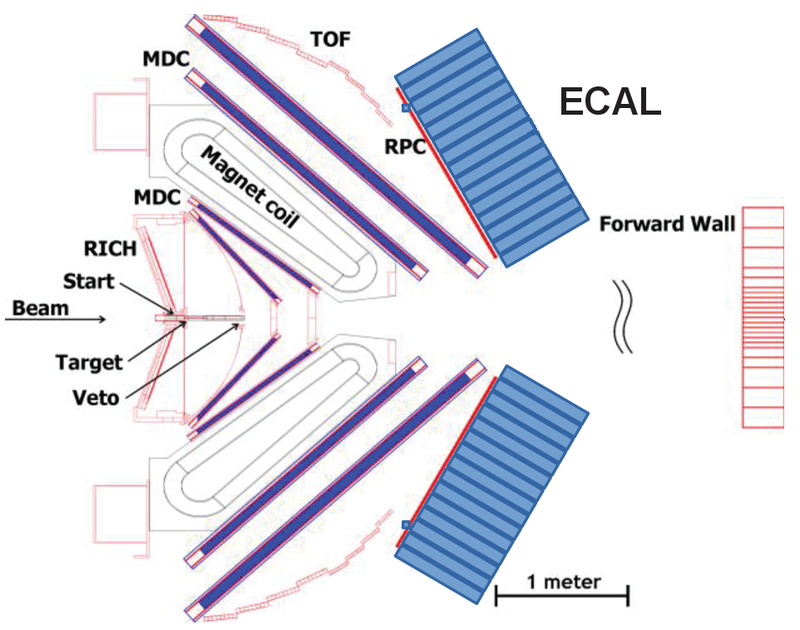
\includegraphics[width=0.75\linewidth]{images/hades_layout.jpg}
\caption{Схема эксперимента HADES}
\label{fig:hades_bmn_layouts}
\end{center}
\end{figure}

\subsection{ Мишень }

Мишень, на которой происходит взаимодействия ускоренных ядер представляет из себя 15 каптоновых полосок, закрепленных на углеволоконной трубке.
На каптоновые полоски толщиной 7~мкм наклеены диски из золота (серебра) толщиной 25~мкм.
Расстояние между полосками составляет 4 мм. 
Общая толщина мишени --- 375~мкм, что соответствует общей вероятности взаимодействия в 1.5\%.
Фотография мишени приведена на рис.~\ref{fig:hades_target}. 
%
\begin{figure}[ht]
\begin{center}
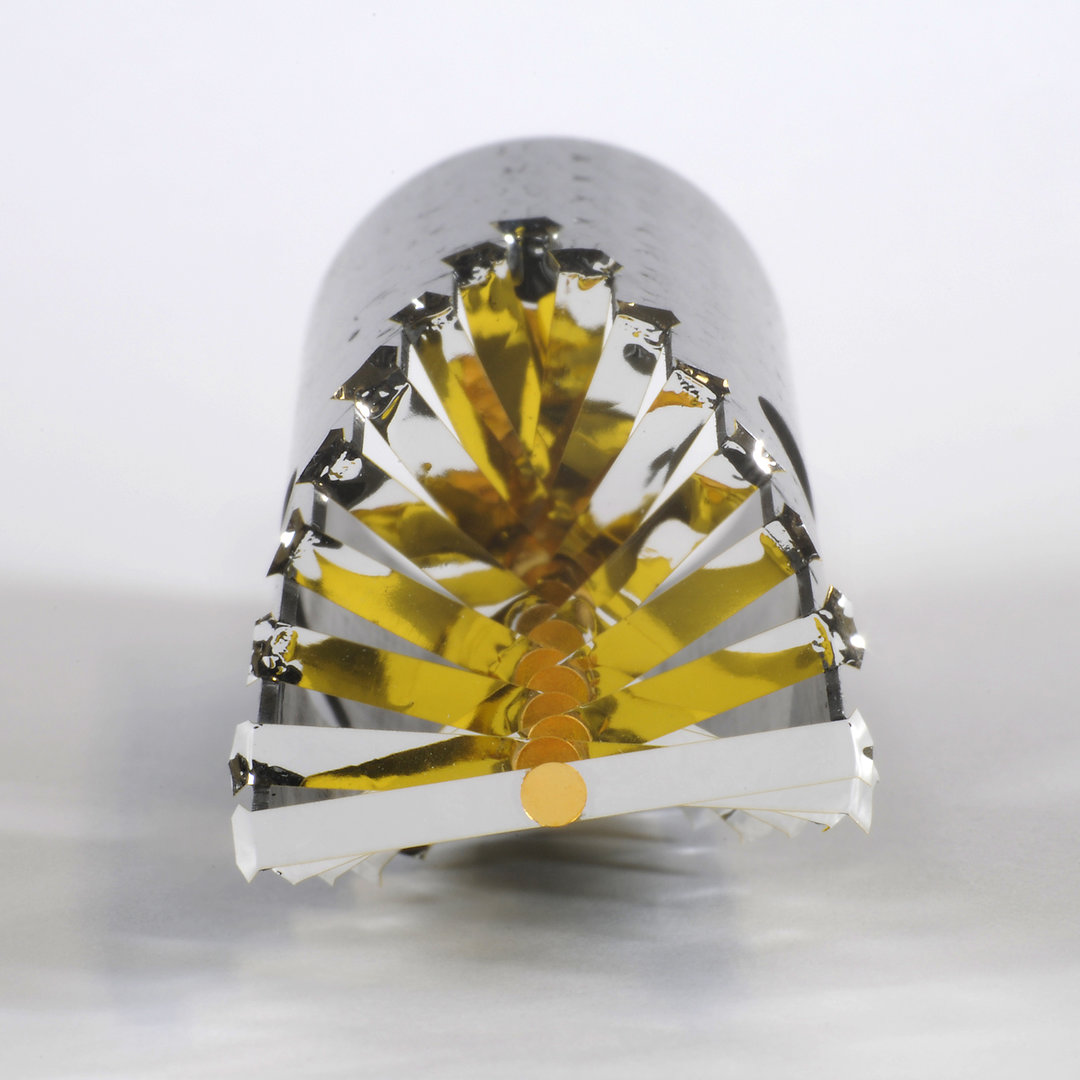
\includegraphics[width=0.55\linewidth]{images/hades_target.jpg}
\caption{ Фотография мишени для сеанса Au~+~Au при энергии 1.23$A$~ГэВ.  }
\label{fig:hades_target}
\end{center}
\end{figure}

\subsection{ Магнитный спектрометр }

Магнитный спектрометр состоит из 6 тороидальных сверхпроводящих магнитов и 24 многопроволочных дрейфовых камер (MDC).
В каждом из 6 секторов две плоскости MDC располагаются до магнита и две --- после. 
Реконструкция импульса производится посредством итеративного решения уравнения движения частиц в локальном магнитном поле при помощи метода Рунге-Кутта.
Заряд частицы определяется по отклонению частицы в магнитном поле: положительно заряженные частиц отклоняются, уменьшая значения полярного угла $\theta$, отрицательно заряженные --- увеличивают значения полярного угла.
Реконструкция импульса может выполняться для большого окна полярных углов в широком диапазоне $p$: от 0.1 до 2 ГэВ/c.
Магнитное поле позволяет измерять импульсы заряженных частиц с разрешением для электронов с энергией 0.15~МэВ $\Delta p/p \approx$ 2\% и протонов с энергией около 1~ГэВ $\Delta p/p \approx$ 4\%.  

\subsection{ Магнит }

Магнитное поле создаётся при помощи сверхпроводящего магнита ISLE, который состоит из 6 секторов, которые в первом приближении отклоняют заряженные частицы, изменяя лишь их полярный угол $\theta$.
При максимальной силе тока $I$=3500~А, максимум магнитного поля в 3 Тл достигается на краях магнита, а в центре сектора составляет 0.9 Тл.
Магнит фокусирует положительно заряженные частиц в направлении оси Z.
Сверхпроводящие катушки состоят из ниобий-титанового сплава, инкапсулированного в медную матрицу.
Медная матрица необходима для механической стабильности конструкции.
Вся сборка упакована в катушки, окруженные аллюминиевым корпусом, который предотвращает механические повреждения в случае внезапного отключения магнитного поля.
Катушки окружены системой охлаждения работающей на жидком азоте при температуре 85~К.
Токопроводящие эллементы дополнительно охлаждаются однофазным гелием при температуре 4.7~К и давлении 2.8 бар.

\subsection{ Камеры MDC }

Площадь чувствительного материала внутренних камер составляет 0.35 м$^2$, а внешних --- 3.21 м$^2$.
Наименьшая чувствительная единица называется чувствительной ячейкой и представляет из себя плоскость с одной чувствительной и двумя потенциальными проволоками.
Катод и анод сделаны из отожженного алюминия, а чувствительная проволока --- из покрытого золотом вольфрама.
Каждая секция состоит из порядка 1100 чувствительных ячеек, организованных в 6 слоёв, каждый из которых повёрнут на 20 градусов друг относительно друга ($\pm0^{\circ}$, $\pm20^{\circ}$, $\pm40^{\circ}$).
Такая организация чувствительного объема позволяет достичь равномерного разрешения по азимутальному (85-125 мкм) и полярному (35-50 мкм) углам.
Первый слой MDC заполнен смесью газов Ar+CO$_{2}$ в пропорциях 70:30.
Оставшиеся три слоя работают на смеси аргона и изобутана. 
Заряженная частица, пролетая через чувствительную зону детектора ионизирует газ, и высвобожденные электроны дрейфуют в сторону чувствительной проволоки.
Собранный заряд детектируется и восстанавливается пространственная координата в которой произошла ионизация газа.

\subsection{START и VETO детекторы}

START и VETO детекторы предназначены для детектирования событий столкновения ядер.
START и VETO используются для регистрации времени столкновения $T_0$ и выработки триггеров.
Совместно с времяпролётными детекторами TOF и RPC, START и VETO позволяют измерять время пролёта заряженных частиц.
Детектор VETO был разработан для подавления эффекта pile-up, когда на мишени происходит более одного взаимодействия.
Детектор имеет малую толщину, приблизительно 60 мкм, и состоит из алмазов, покрытых тонкой плёнкой металла. 
START детектор в свою очередь собран из алмазов с металлическим напылением, нанесенных тонким слоем на полоски из хромированного золота.
Всего 16 полосок шириной 200 мкм с интервалом в 90 мкм обеспечивают высокую точность регистрации налетающего ядра по $x$ и $y$.

\subsection{Времяпролётный детекторы TOF и RPC}

Времяпролётный детектор TOF состоит из 384 сцинтилярных стержней из поливинилтолуола, который обладает малой длиной ослабления света, высоким сцинтиляционным выходом и коротким временем распада.
Поперечные размеры внутренних стержней составляют $20 \times 20$ мм$^2$ и внешних --- $30\times30$ мм$^2$.
Проходя через сцинтиляционный стержень, заряженная частица возбуждает атомы чувствительного материала, которые затем возвращаются в основное состояние через эмиссию света.
Излученный свет распространяется в оба конца детектора, где считывается при помощи двух фотоумножителей.
По разности времён регистрации света на двух концах сцинтиляционного стержня затем рассчитывается $x$-координата попадания частицы.
Также по амплитуде сигнала рассчитываются энергопотери заряженной частицы при прохождении через материал детектора.

Для увеличения аксептанса времяпролетной системы, ближе к оси пучка за детекторами TOF находятся 6 резистивных плоскостных детекторов (RPC). 
Каждая секция состоит из двух частично перекрывающихся слоёв, в каждом из которых находится 31 полоска RPC.
Каждый RPC собран из чередующихся слоев аллюминиевых электродов и изолятора --- стекла --- в газовом объеме, заполненном смесью $SF_6$ и $C_2H_2F_4$.
Заряженные частицы ионизируют газ и дельта-электроны ускоряются магнитным полем в сторону анода, создавая электронную лавину.

\subsection{ Трекинговая система }

Трекинговая система HADES, предназначенная для реконструкции траекторий заряженных частиц, состоит из четырёх плоскостей многопроволочных дрейфовых камер (MDC).
Для измерения импульса заряженных частиц, между второй и третьей плоскостями, располагается сверхпроводящий магнит, отклоняющий проходящие через него частицы.
На рис.~\ref{fig:hades_tracking} схематически изображена трекинговая система эксперимента HADES.
Треки заряженных частиц совмещаются из траекторий в плоскостях I и II, и III и IV методом Рунге-Кутта.
Импульс заряженной частицы восстанавливается по отклонению в магнтином поле между плоскостями II и III 
%
\begin{figure}[ht]
\begin{center}
    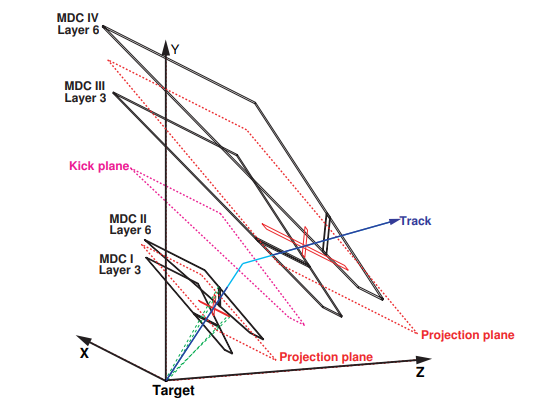
\includegraphics[width=0.55\linewidth]{images/hades_tracking_system.png}
    \caption{Схмеатическое изображение трекинговой системы эксперимента HADES.}
    \label{fig:hades_tracking}
\end{center}
\end{figure}

\subsection{Передний годоскоп Forward Wall}

Для регистрации фрагментов сталкивающихся ядер, взаимодействовавших с областью перекрытия лишь упруго (спектаторы), спектрометр HADES оборудован годоскопом FW.
Детектор имеет модульную структуру и способен измерять заряд фрагментов-спектаторов.
Размер модулей годоскопа увеличивается от центральных к периферическим и составляет $40\times40$, $80\times80$ и $160\times160$~мм$^2$ соответственно.
Схематично, расположение модулей в годоскопе представлено на рис.~\ref{fig:hodo_layout}.
%
\begin{figure}[ht]
\begin{center}
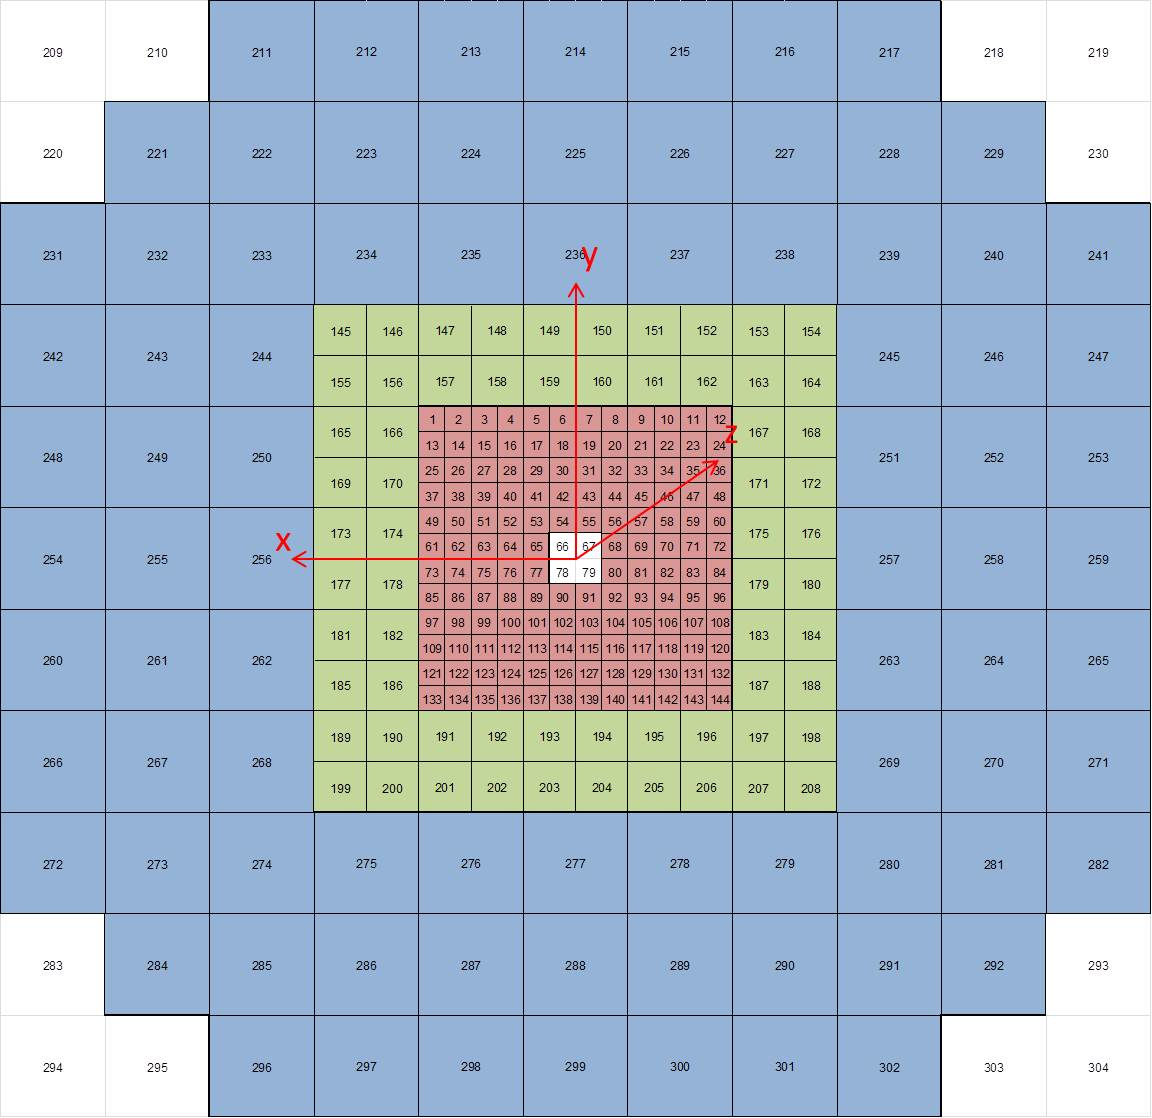
\includegraphics[width=0.55\linewidth]{images/FW_layout.jpg}
\caption{Схема расположения модулей переднего годоскопа FW.}
\label{fig:hodo_layout}
\end{center}
\end{figure}
